\documentclass[english,a4paper,11pt]{report}
\usepackage[utf8]{inputenc}
\usepackage[T1]{fontenc}
\PassOptionsToPackage{english}{babel}
\usepackage{graphicx}
\usepackage{fullpage}
\usepackage{eso-pic}
\usepackage{cite}
\usepackage{wrapfig}
\usepackage{url}
\usepackage[english]{babel}
\usepackage{fancyhdr}
\usepackage{hyperref}
\usepackage[lastpage,user]{zref}
\cfoot{\thepage\ of \zpageref{LastPage}}
\pagestyle{fancy}
\usepackage[headsep=1cm,headheight=61pt,footskip=3cm]{geometry}


\newcommand{\HRule}{\rule{\linewidth}{0.5mm}}
 \newcommand{\ts}{\textsuperscript}
\newcommand{\blap}[1]{\vbox to 0pt{#1\vss}}
\newcommand\AtUpperLeftCorner[3]{%
  \put(\LenToUnit{#1},\LenToUnit{\dimexpr\paperheight-#2}){\blap{#3}}%
}
\newcommand\AtUpperRightCorner[3]{%
  \put(\LenToUnit{\dimexpr\paperwidth-#1},\LenToUnit{\dimexpr\paperheight-#2}){\blap{\llap{#3}}}%
}
\newcommand\AtLowerRightCorner[3]{%
  \put(\LenToUnit{\dimexpr\paperwidth-#1},\LenToUnit{#2}){#3}%
}
 
\title{\LARGE{Automation and robotic project 1}}
\author{\textsc{Breton-Belz} Emmanuel - UNISA 2015 - 2016}
\date{\today}
\makeatletter

\renewcommand{\headrulewidth}{1pt}
\fancyhead[C]{\@author} 
\fancyhead[L]{\leftmark}
\fancyhead[R]{
\includegraphics[width=2cm]{images_not_compressed/unisaLogo.jpg}}
\addto\captionsenglish{
  \renewcommand{\contentsname}
    {Table of contents}
}
\renewcommand{\footrulewidth}{1pt}
\fancyfoot[R]{\leftmark}
		 
\begin{document}
	%\setcounter{tocdepth}{4}
	
	\begin{titlepage}
	\begin{center}
	        \vspace*{6cm}
	        \textsc{\@title}
	        \HRule
	        \vspace*{0.5cm}
	        \large{\@author} 
	 \end{center}
	 
	
	    \AddToShipoutPicture{%
	      \AtUpperLeftCorner{1.5cm}{1cm}{
\includegraphics[width=4cm]{images_not_compressed/unisaLogo.jpg}}
	     }
	     
	\begin{center}
		\vspace*{2.5cm}
		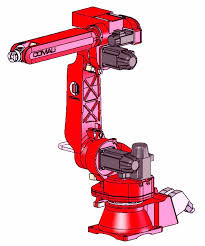
\includegraphics[width=8cm]{images_not_compressed/smart5.jpg}
	\end{center}
	 

	
	\end{titlepage}
	\ClearShipoutPicture
	
	\tableofcontents
	\newpage
	
	
	\chapter{Introduction}
		
	In this project we apply the theory seen in 

	\listoffigures
	
\end{document}